% \documentclass[aspectratio=169,notes]{beamer}
\documentclass[aspectratio=169]{beamer}
\usetheme[faculty=phil]{fibeamer}
\usepackage{polyglossia}
\setmainlanguage{english} %% main locale instead of `english`, you
%% can typeset the presentation in either Czech or Slovak,
%% respectively.
\setotherlanguages{russian} %% The additional keys allow
%%
%%   \begin{otherlanguage}{czech}   ... \end{otherlanguage}
%%   \begin{otherlanguage}{slovak}  ... \end{otherlanguage}
%%
%% These macros specify information about the presentation
\title[MaM]{Mechanics and Machines, MAN 1} %% that will be typeset on the
\subtitle{How to make such parts?
\\ \  \\ \ 
    } %% title page.
\author{Oleg Bulichev}
%% These additional packages are used within the document:
\usepackage{ragged2e}  % `\justifying` text
\usepackage{booktabs}  % Tables
\usepackage{tabularx}
\usepackage{tikz}      % Diagrams
\usetikzlibrary{calc, shapes, backgrounds}
\usepackage{amsmath, amssymb}
\usepackage{url}       % `\url`s
\usepackage{listings}  % Code listings
% \usepackage{subfigure}
\usepackage{floatrow}
\usepackage{subcaption}
\usepackage{mathtools}
\usepackage{todonotes}
\usepackage{fontspec}
\usepackage{multicol}
\usepackage{pdfpages}
\usepackage{wrapfig}
\usepackage{animate}
\usepackage{booktabs}
\usepackage{multirow}
% \usepackage{graphicx}
\usepackage{colortbl}

\graphicspath{{resources/}}
\frenchspacing

\setbeamertemplate{caption}[numbered]
\usetikzlibrary{graphs}

% \usepackage[backend=biber,style=ieee,autocite=footnote]{biblatex}
% \addbibresource{biblio.bib}
% \DefineBibliographyStrings{english}{%
%   bibliography = {References},}

\newcommand{\oleg}[2][] {\todo[color=red, #1] {OLEG:\\ #2}}
\newcommand{\fbckg}[1]{\usebackgroundtemplate{\includegraphics[width=\paperwidth]{#1}}}%frame background

\usepackage[framemethod=TikZ]{mdframed}
\newcommand{\dbox}[1]{
\begin{mdframed}[roundcorner=3pt, backgroundcolor=yellow, linewidth=0]
\vspace{1mm}
{#1}
\vspace{1mm}
\end{mdframed}
}

\begin{document}
\setlength{\abovedisplayskip}{0pt}
\setlength{\belowdisplayskip}{0pt}
\setlength{\abovedisplayshortskip}{0pt}
\setlength{\belowdisplayshortskip}{0pt}

\fbckg{fibeamer/figs/title_page.png}
\frame[c]{\setcounter{framenumber}{0}
    \usebeamerfont{title}%
    \usebeamercolor[fg]{title}%
    \begin{minipage}[b][6.5\baselineskip][b]{\textwidth}%
        \textcolor{black}{\raggedright\inserttitle}
    \end{minipage}
    % \vskip-1.5\baselineskip

    \usebeamerfont{subtitle}%
    \usebeamercolor[fg]{framesubtitle}%
    \begin{minipage}[b][3\baselineskip][b]{\textwidth}
        \raggedright%
        \insertsubtitle%
    \end{minipage}
    \vskip.25\baselineskip
}
%   \frame[c]{\maketitle}

\fbckg{fibeamer/figs/common.png}

\note{\scriptsize
\ 
}

\begin{frame}[c]{Shaft (Вал)}
\framesubtitle{}
    \vspace{-0.6cm}
    \begin{figure}[H]
        \centering\includegraphics[height=6cm,width=1\textwidth,keepaspectratio]{shaft.png}
        \label{fig:shaft.png}
    \end{figure}
\end{frame}

\begin{frame}[c]{Shaft}
\framesubtitle{}
    \LARGE \centering
    \textbf{Possible operations: } \\ 
    Turning-milling\\
\end{frame}

\begin{frame}[c]{Part of a body connector (StriRus)}
\framesubtitle{}
    \vspace{-0.6cm}
    \begin{figure}[H]
        \begin{subfigure}{0.49\textwidth}
            \centering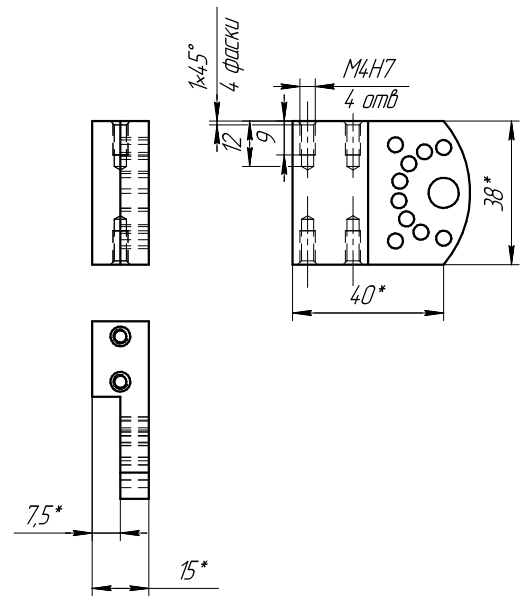
\includegraphics[height=6cm,width=1\textwidth,keepaspectratio]{stri_1.png}
            % \caption{capture1}
            \label{fig:stri_1.png}
        \end{subfigure}
        \begin{subfigure}{0.49\textwidth}
            \centering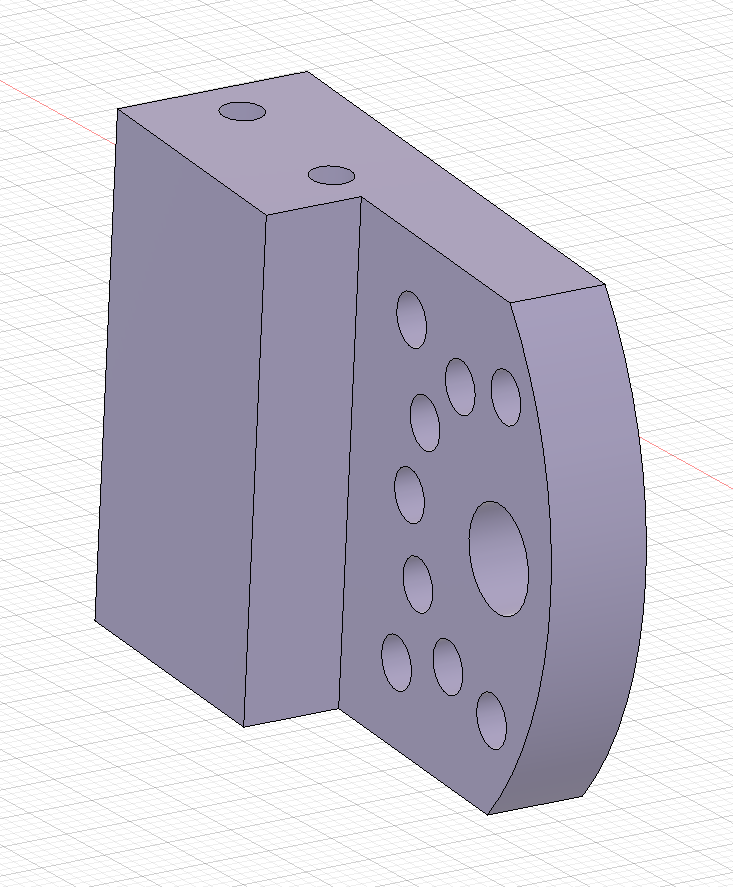
\includegraphics[height=6cm,width=1\textwidth,keepaspectratio]{stri1_det.png}
            % \caption{capture2}
            \label{fig:stri1_det.png}
        \end{subfigure}
    
    % \caption{capture_main}
    % \label{fig:}
    \end{figure}
\end{frame}

\begin{frame}[c]{Part of a body connector}
    \framesubtitle{}
        \LARGE \centering
        \textbf{Possible operations: } \\ 
        3D milling\\
        3D printing
    \end{frame}

\begin{frame}[c]{Plate}
\framesubtitle{}
    \vspace{-0.6cm}
    \begin{figure}[H]
        \centering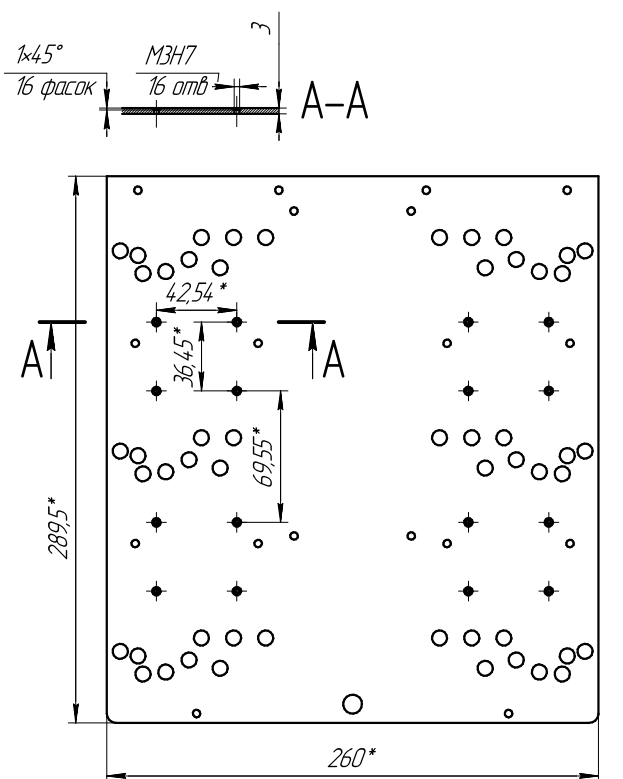
\includegraphics[height=6cm,width=1\textwidth,keepaspectratio]{stri_2.png}
        \label{fig:stri_2.png}
    \end{figure}
\end{frame}

\begin{frame}[c]{Plate}
    \framesubtitle{}
        \LARGE \centering
        \textbf{Possible operations: } \\ 
        3D milling\\
        laser cutting\\
    \end{frame}

\begin{frame}[c]{Car shell for sensors}
\framesubtitle{}
    \vspace{-0.6cm}
    \begin{figure}[H]
        \centering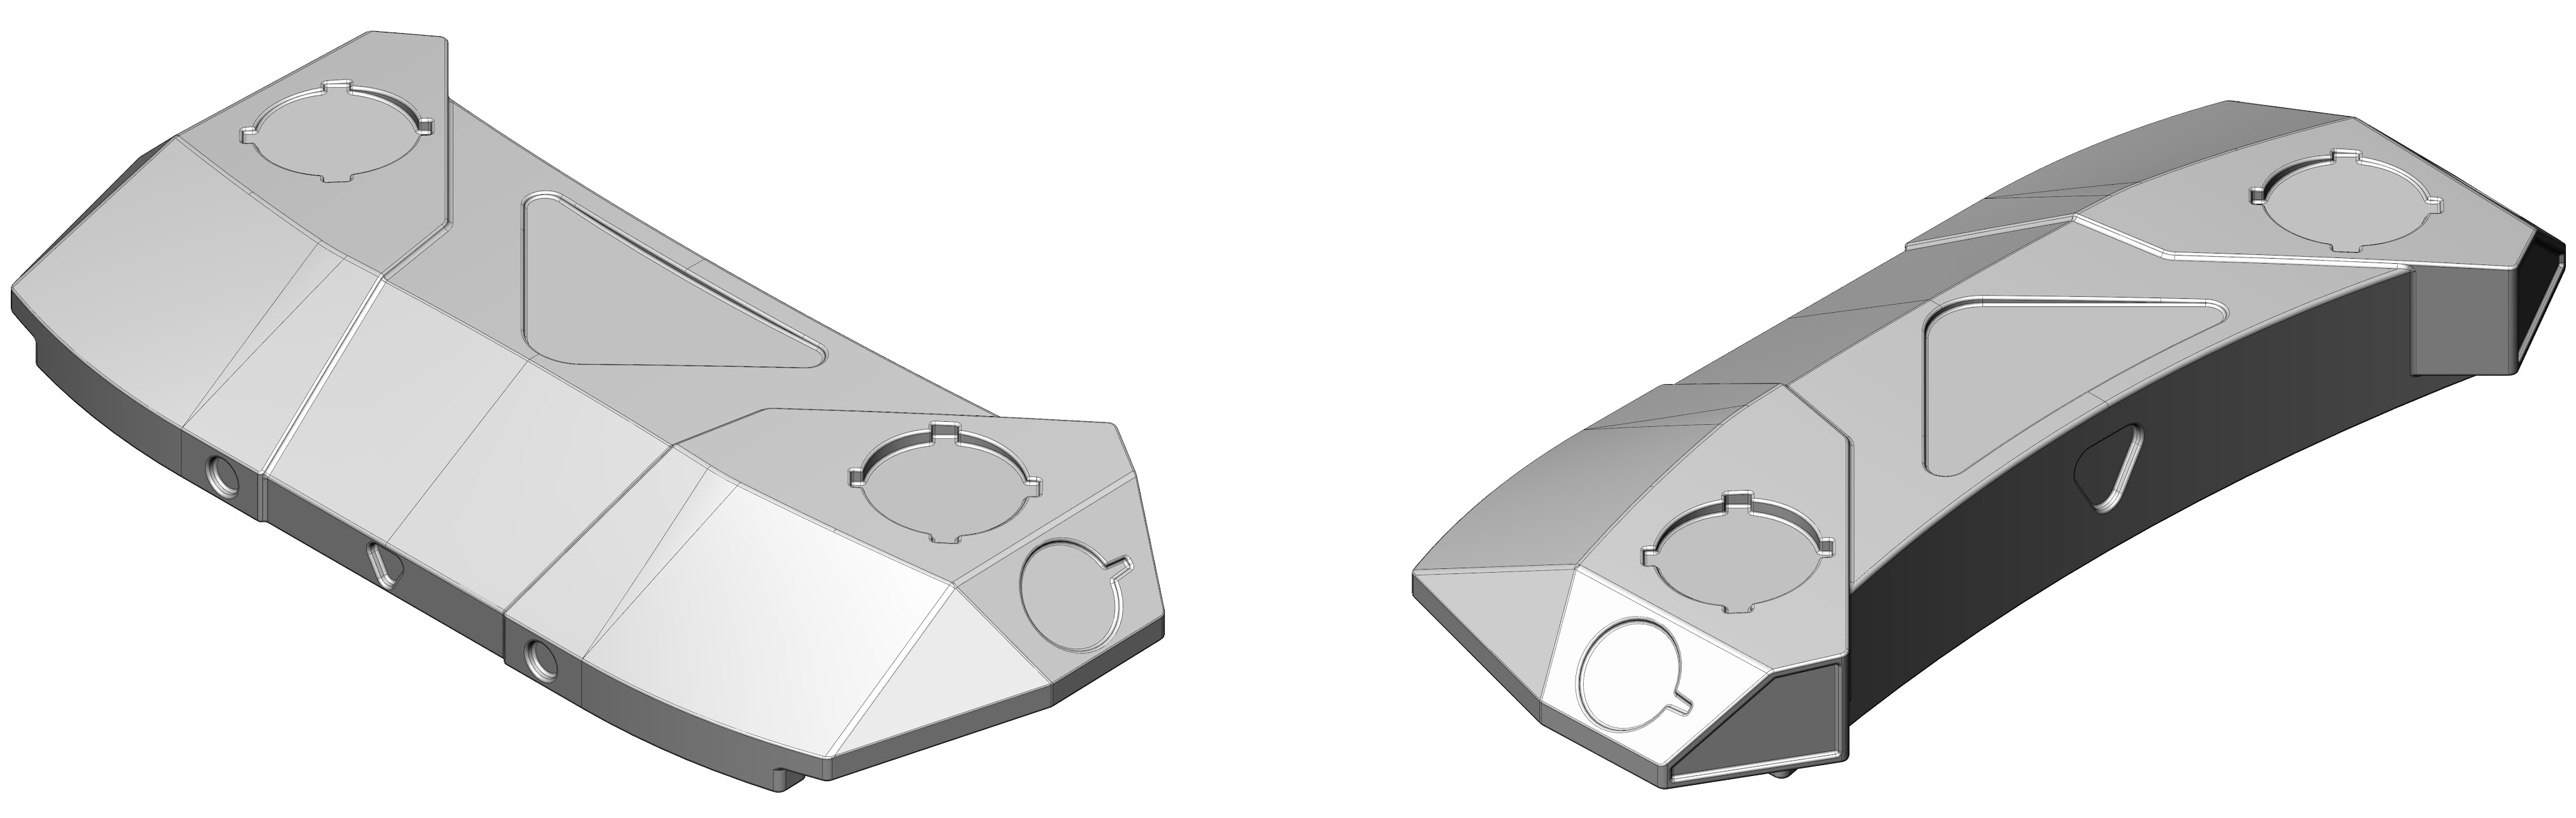
\includegraphics[height=6cm,width=1\textwidth,keepaspectratio]{Image_15.jpg}
        \label{fig:Image_15.jpg}
    \end{figure}
\end{frame}

\begin{frame}[c]{Car shell for sensors}
    \framesubtitle{}
        \LARGE \centering
        \textbf{Possible operations: } \\ 
        Casting / Molding\\
    \end{frame}

\begin{frame}[c]{Damascus Knife}
\framesubtitle{}
    \vspace{-0.6cm}
    \begin{figure}[H]
        \centering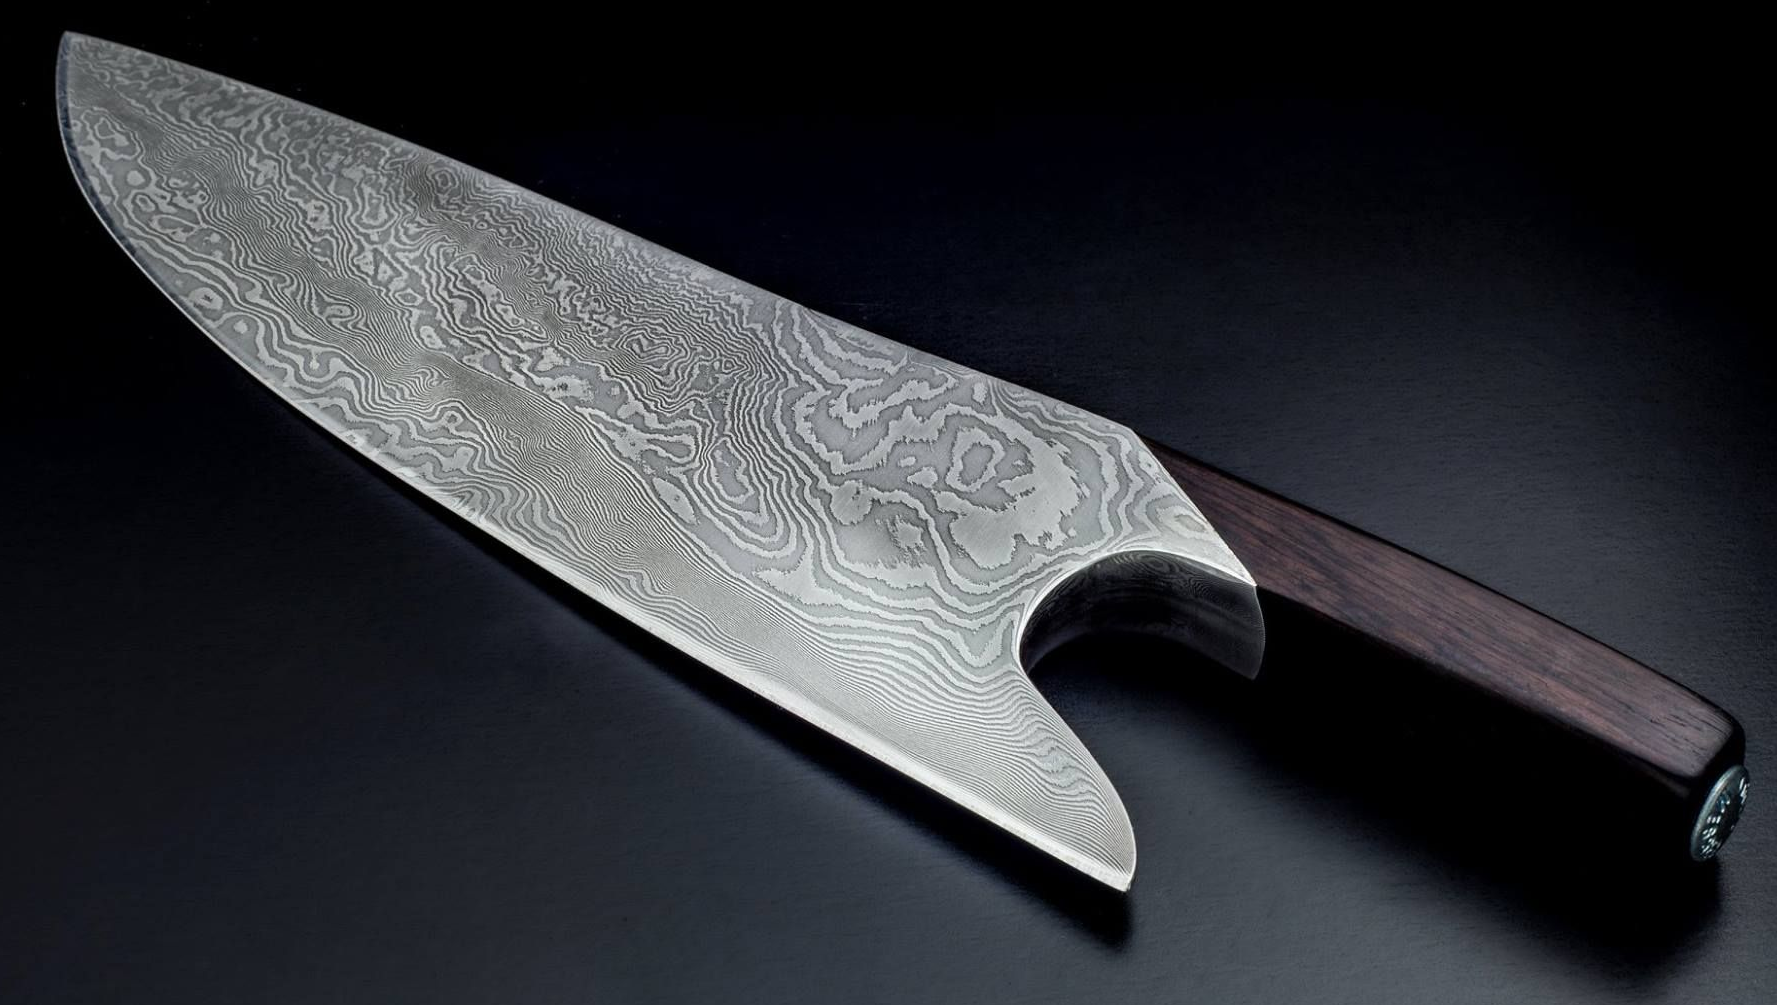
\includegraphics[height=6cm,width=1\textwidth,keepaspectratio]{Image_17.png}
        \label{fig:Image_17.png}
    \end{figure}
\end{frame}

\begin{frame}[c]{Damascus Knife}
    \framesubtitle{}
        \LARGE \centering
        \textbf{Possible operations: } \\ 
        Forge-welding + acid etch with ferric chloride\\
    \end{frame}

\begin{frame}[c]{Cast-iron (чугун) frypan}
\framesubtitle{}
    \vspace{-0.6cm}
    \begin{figure}[H]
        \centering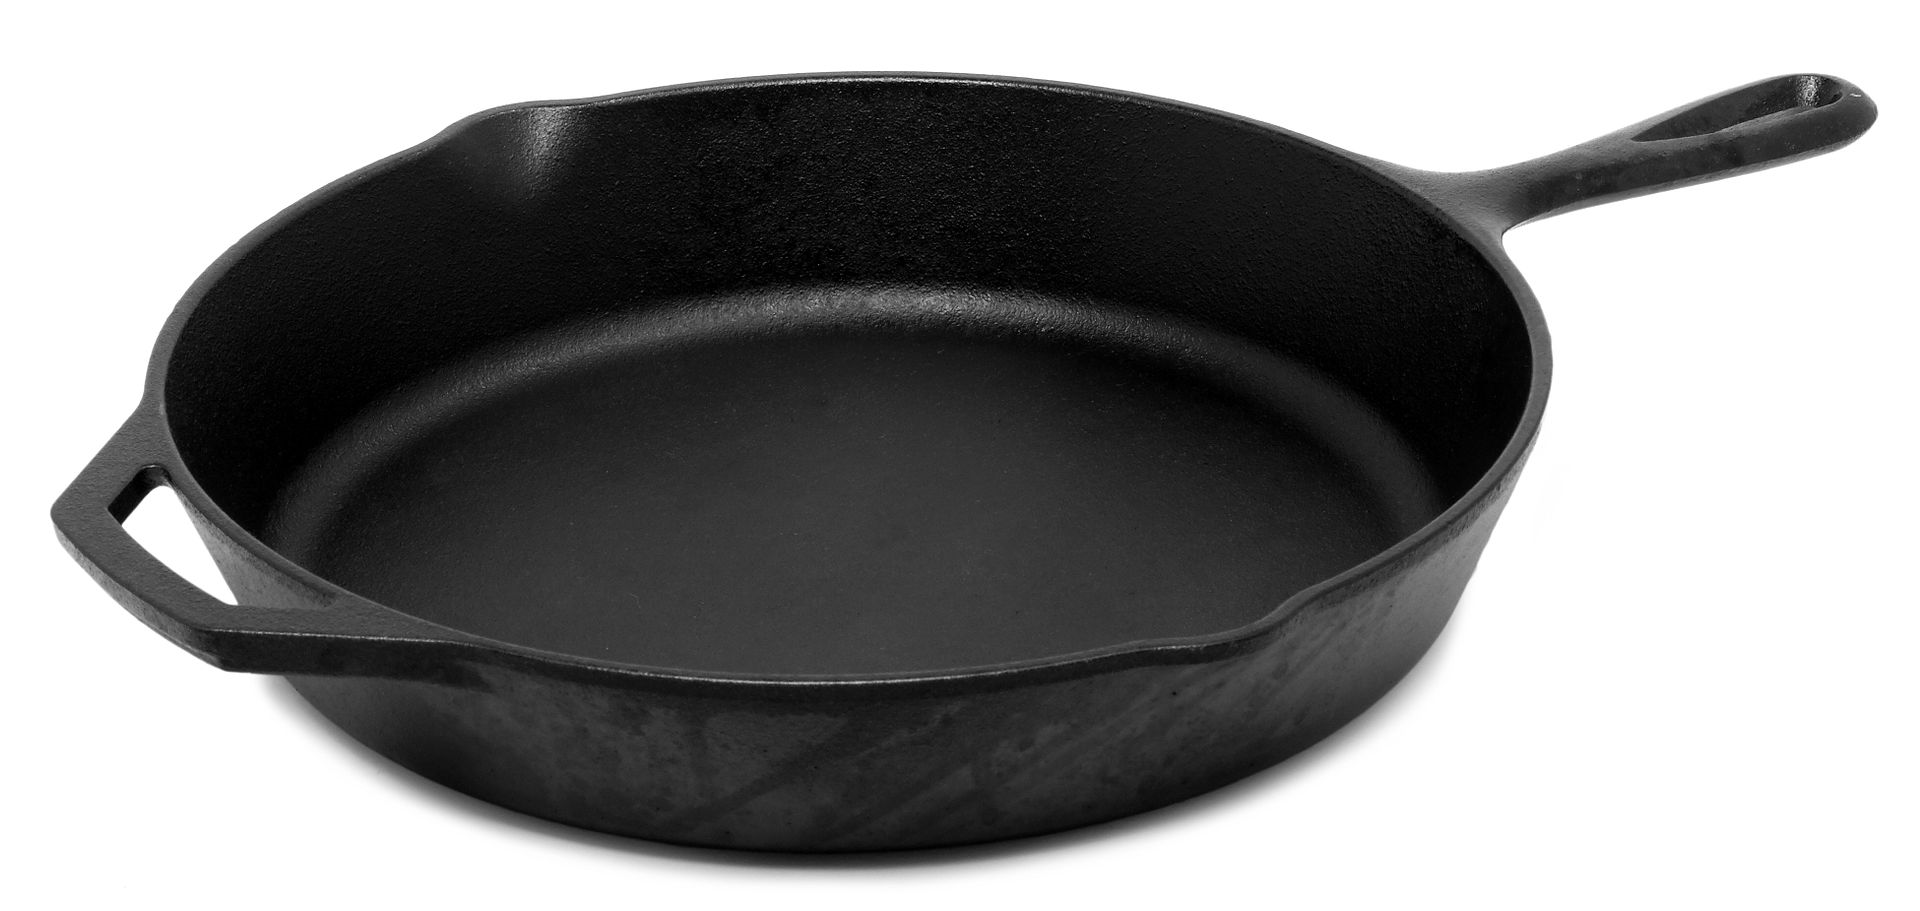
\includegraphics[height=6cm,width=1\textwidth,keepaspectratio]{cast_iron.png}
        \label{fig:cast_iron.png}
    \end{figure}
\end{frame}

\begin{frame}[c]{Cast-iron (чугун) frypan}
    \framesubtitle{}
        \LARGE \centering
        \textbf{Possible operations: } \\ 
        Casting\\
    \end{frame}

\begin{frame}[c]{Turbocharger impeller Крыльчатка турбокомпрессора}
\framesubtitle{}
    \vspace{-0.6cm}
    \begin{figure}[H]
        \centering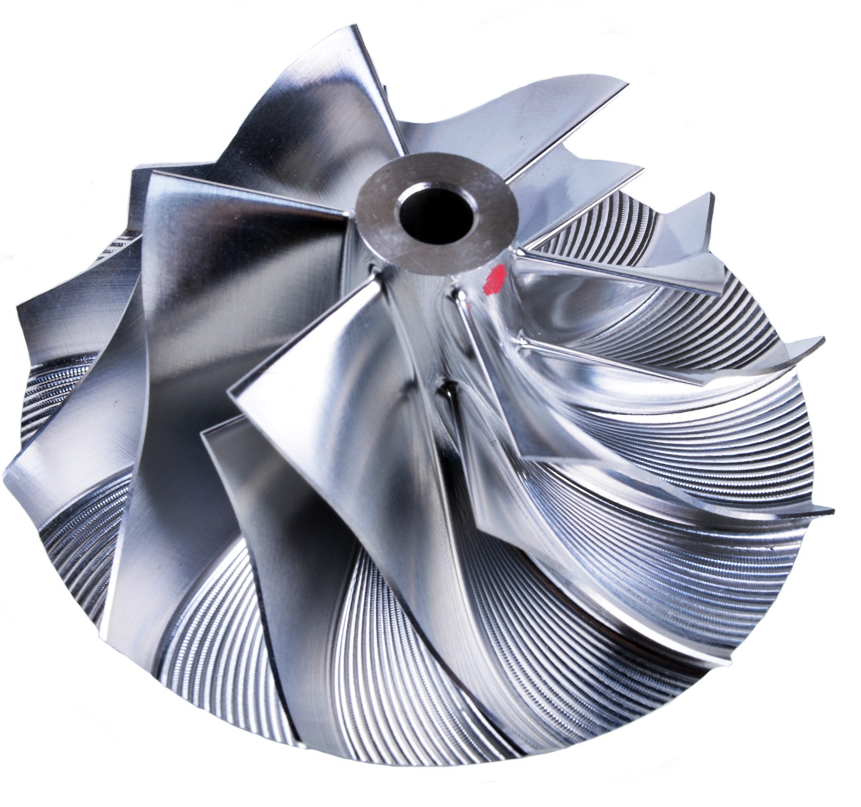
\includegraphics[height=6cm,width=1\textwidth,keepaspectratio]{tourbin.png}
        \label{fig:tourbin.png}
    \end{figure}
\end{frame} 

\begin{frame}[c]{Turbocharger impeller}
    \framesubtitle{}
        \LARGE \centering
        \textbf{Possible operations: } \\ 
        4D(5D) milling\\
        3D metal printing
    \end{frame}

\begin{frame}[c]{T-Slotted Framing Rails (Алюм. профиль)}
\framesubtitle{}
    \vspace{-0.6cm}
    \begin{figure}[H]
        \centering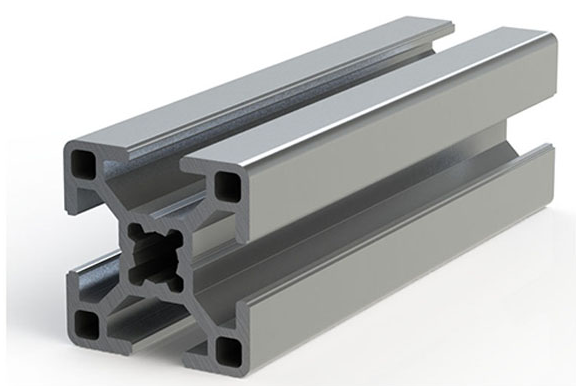
\includegraphics[height=6cm,width=1\textwidth,keepaspectratio]{t_slot.png}
        \label{fig:t_slot.png}
    \end{figure}
\end{frame}

\begin{frame}[c]{T-Slotted Framing Rails}
    \framesubtitle{}
        \LARGE \centering
        \textbf{Possible operations: } \\ 
        Extruding\\
    \end{frame}

\begin{frame}[c]{Toy}
\framesubtitle{}
    \vspace{-0.6cm}
    \begin{figure}[H]
        \centering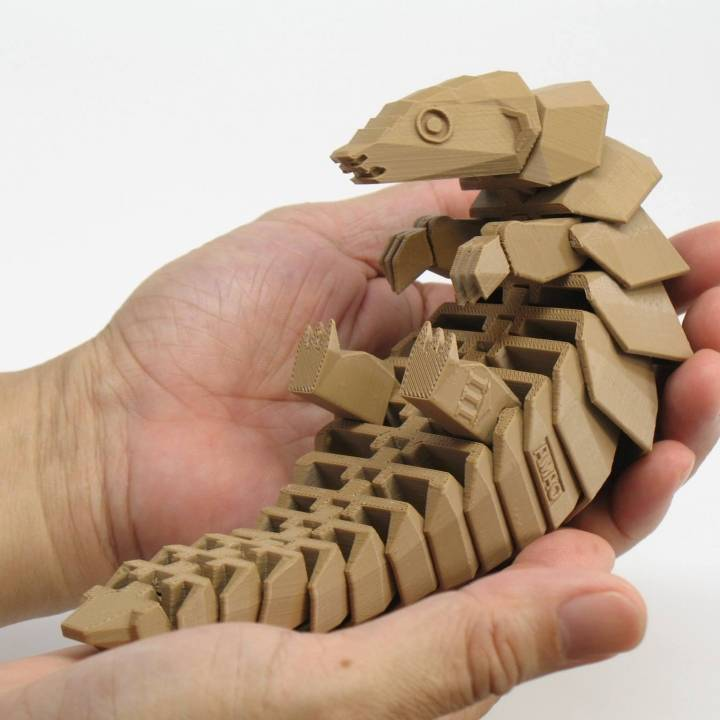
\includegraphics[height=6cm,width=1\textwidth,keepaspectratio]{toy.png}
        \label{fig:toy.png}
    \end{figure}
\end{frame}

\begin{frame}[c]{Toy}
    \framesubtitle{}
        \LARGE \centering
        \textbf{Possible operations: } \\ 
        3D printer\\
        Casting (very expensive)
    \end{frame}

\begin{frame}[c]{Mounting bracket (Уголок)}
\framesubtitle{}
    \vspace{-0.6cm}
    \begin{figure}[H]
        \centering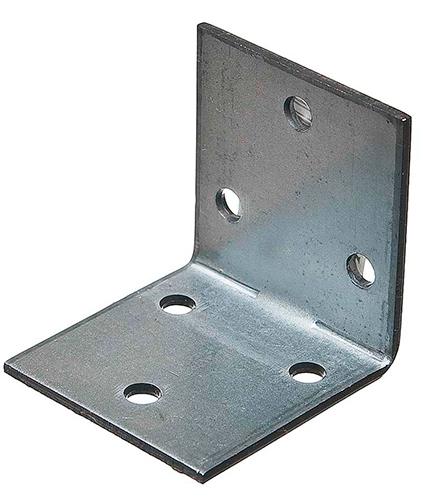
\includegraphics[height=6cm,width=1\textwidth,keepaspectratio]{angle.png}
        \label{fig:angle.png}
    \end{figure}
\end{frame}

\begin{frame}[c]{Mounting bracket}
    \framesubtitle{}
        \LARGE \centering
        \textbf{Possible operations: } \\ 
        Stamping (Pressing) and Bending\\
        3D printing
    \end{frame}

\begin{frame}[c]{Stoneware (гранитная) plate}
\framesubtitle{}
    \vspace{-0.6cm}
    \begin{figure}[H]
        \centering
\includegraphics[height=6cm,width=1\textwidth,keepaspectratio]{water.jpg}
        \label{fig:water.jpg}
    \end{figure}
\end{frame}

\begin{frame}[c]{Stoneware plate}
    \framesubtitle{}
        \LARGE \centering
        \textbf{Possible operations: } \\ 
        Water jet cutting\\
    \end{frame}

\begin{frame}[c]{Metal small figures}
\framesubtitle{}
    \vspace{-0.6cm}
    \begin{figure}[H]
        \centering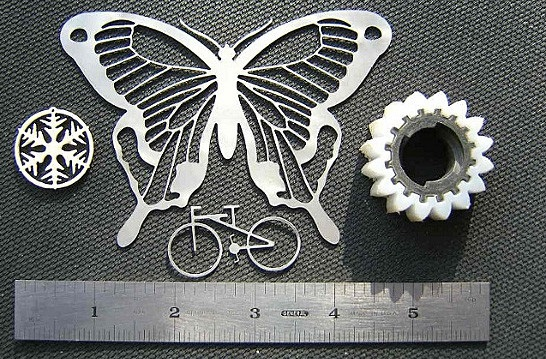
\includegraphics[height=6cm,width=1\textwidth,keepaspectratio]{lazer.jpeg}
        \label{fig:lazer.jpeg}
    \end{figure}
\end{frame}

\begin{frame}[c]{Metal small figures}
    \framesubtitle{}
        \LARGE \centering
        \textbf{Possible operations: } \\ 
        laser cutting\\
        3D SLA printer\\
        Electrical discharge machining
    \end{frame}

\begin{frame}[c]{Rusty pin}
\framesubtitle{}
    \vspace{-0.6cm}
    \begin{figure}[H]
        \centering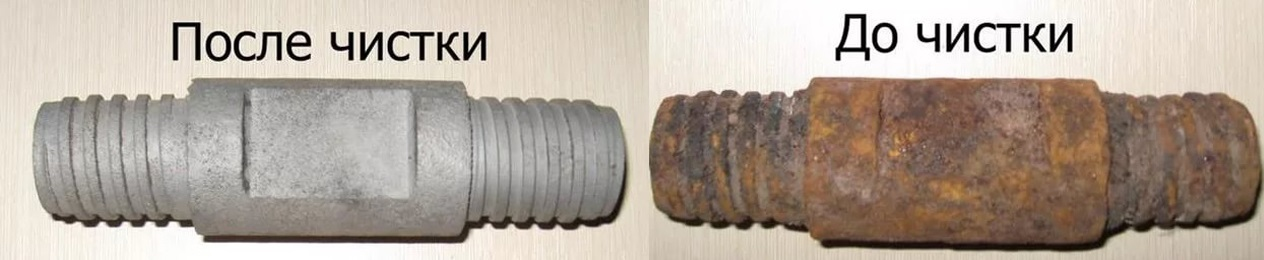
\includegraphics[height=6cm,width=1\textwidth,keepaspectratio]{sand_blazing.jpg}
        \label{fig:sand_blazing.jpg}
    \end{figure}
\end{frame}

\begin{frame}[c]{Rusty pin}
    \framesubtitle{}
        \LARGE \centering
        \textbf{Possible operations: } \\ 
        Turning + Sandblasting (пескоструй)\\
    \end{frame}

\fbckg{fibeamer/figs/last_page.png}
\frame[plain]{}

\end{document}